\documentclass[12pt,a4paper]{article}

% Packages
\usepackage[margin=0.6in]{geometry} 
\usepackage{setspace} 
\usepackage{titlesec}
\usepackage{graphicx}
\usepackage{booktabs}
\newcommand{\ra}[1]{\renewcommand{\arraystretch}{#1}}
\graphicspath{{./Images/}}
\usepackage[colorlinks=true,linkcolor=black,citecolor=red,urlcolor=red]{hyperref}
\usepackage{amsmath}
\usepackage[numbers,link]{natbib}


% Title formatting
\titleformat{\section}[block]{\large\bfseries}{\thesection}{1cm}{}
\usepackage{fancyhdr}
\pagestyle{plain}


\begin{document}

% Title Page
\begin{titlepage}
    \vspace{1cm}
    \centering
    \Huge{\textbf{Research Essay}} \\
    \vspace{1.5cm}
    \large{\textbf{Quantum Resources in the Jaynes-Cummings Model}}\\
    \vspace{1cm}
    \small{Submitted by: Rowan Adeya \\
    Date: \today} \\
    \vspace{1cm}
    \small{\textit{Supervisor: Dr. Alexandra Olaya-Castro}} \\
    \small{\textit{Second Supervisor: Prof. Dan Browne}} \\

    \vspace{5cm}
    


    \vfill
    \normalsize
    University College London
\end{titlepage}

\newpage

\vspace{2cm}
\begin{abstract}
    The Jaynes-Cummings Model (JCM) is a fundamental theoretical framework for describing the interaction between a two-level system and a single quantised mode of a quantum harmonic oscillator. This literature review examines the role and relevance of the JCM, highlighting its applications in cavity QED, circuit QED, and other notable systems. The review also explores the extraction of quantum resources, such as entanglement and coherence, from the JCM, with a focus on widely used measures like von Neumann entropy and relative entropy of coherence. Limitations of the JCM include its breakdown in the ultrastrong coupling regime, and its inapplicability to more than one two-level system or/and quantum harmonic oscillator. Thus, alternative models such as the Rabi and Dicke models are discussed. Furthermore, recent advancements in entanglement preservation, coherence control, and coherence degradation in the JCM are reviewed. We find that the JCM continues to be a valuable framework for understanding simpler quantum systems in the strong and weak coupling regimes, offering clear, reliable predictions. Moreover, the JCM's simplicity and extendability makes it an ideal tool for analysing quantum resources.
\end{abstract}

\newpage

\tableofcontents

\newpage

\section{Introduction} \label{intro}
% Intro to JCM and light description

The quantum description of light-matter interaction is a cornerstone of modern quantum science, underpinning technologies such as quantum computing, communication, and cavity QED. A model which fully captures the dynamics of such systems would allow us to better understand and control quantum phenomena, leading to the development of future quantum technologies. Moreover, we can leverage the simplicity of models to gain easier access to quantum resources (such as entanglement and coherence) that are essential for practical quantum applications.


The quantum description of light-matter interaction can be modelled by a two-level system (TLS) interacting with a quantum harmonic oscillator (QHO). In 1963, Edwin Jaynes and Fred Cummings set out to model a single atom interacting with one mode of a quantized electromagnetic field within an optical cavity using the TLS-QHO model (see figure \ref{fig:1_JCM}) under the Rotating Wave Approximation (RWA) (see section \ref{JCM_apps} for definition) \cite{Context1963-JC_Original}. As such, they formulated the Jaynes-Cummings Model (JCM), which remains one of the simplest and most important models of light-matter interaction. Later in 1985, Walther experimentally verified the JCM, proving its importance in the field of cavity QED \cite{Context1993-JC_Verification}. 
% Applications of JCM 

\begin{figure}[h]
    \centering
    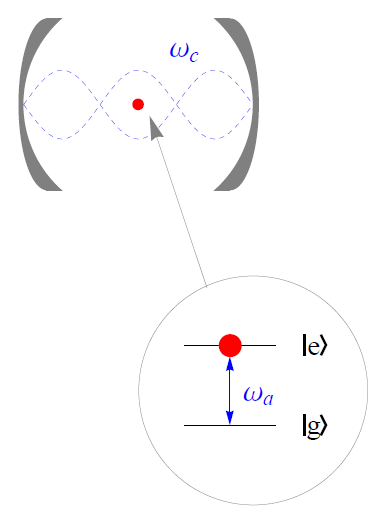
\includegraphics[scale=0.6]{Images/Jaynes-Cummings_model.png}
    \caption{Example of the JCM in the context of cavity QED. The atom, modelled as a TLS with frequency $\omega_a$, is the red dot on the top left. The atom resides in an optical cavity, modelled as a QHO with frequency $\omega_c$. Image adapted from \cite{Image-Prince_JCM}. Used under the terms of the CC BY-SA 3.0 license.}
    \label{fig:1_JCM}
\end{figure}

\vspace{0.4cm}

Presently, the JCM has been extended to other various areas of physics research, including circuit QED \cite{Context2018-Supercond_qubit}, tunnelling phenomena in photonic crystals \cite{Context2012-Tunneling_photons}, and trapped ion physics \cite{Context1992-Trapped_ions}. On the other hand, the simplicity of this model is limiting. The model fails in certain scenarios, such as in the ultra-strong coupling regime in cavity QED, in systems with more than one TLS or multiple modes of the QHO, and when the RWA is no longer valid \cite{General2024-JC_overview}. The Quantum Rabi Model provides a solution to the this problem by including terms originally ignored by the RWA \cite{General2024-JC_overview}. The Dicke Model generalises both the JCM and Rabi models by allowing for more than one TLS and/or QHO, and by not employing the RWA \cite{General2024-JC_overview}. Despite the existence of more sophisticated models, the approximations made in the JCM are still valid for describing many scenarios, making it a popular model to this day. 
% Intro and importance of QResources

Although more complex models exist, the analytical solvability of the JCM makes it a valuable tool for gaining further insights into light-matter interaction. Understanding how quantum resources manifest within this model provides a foundation for exploring more advanced quantum phenomena. This has led to the study of two key quantum resources: entanglement and coherence, both of which play essential roles in quantum communication and quantum computation, among other applications. Entanglement is a basis-independent measure of the quantum correlation between subsystems of a composite system, indicating how much the system's state deviates from a separable (product) state \cite{Entanglement2009-Definition}. Similarly, coherence is a basis-\textit{dependent} measure that describes the ability of a system to remain in a quantum superposition state, and quantifies how well quantum states preserve the phase relationships between different basis states \cite{Coherence2017-Colloquium}. 

As quantum technology progresses, achieving precise control over quantum states has become increasingly important for practical applications. In the context of the TLS-QHO model, entanglement and coherence are key resources that enable both the theoretical exploration and experimental control of the system. Entanglement in the TLS-QHO naturally arises from the coupling of the TLS and QHO \cite{Entanglement2009-REE_VNapplied}. On the other hand, coherence directly affects the stability and controllability of the system \cite{Coherence2020-JCMapplied}.  By harnessing these quantum resources, the TLS-QHO model provides a versatile framework for studying and developing future quantum technologies. Given its well-established analytical techniques, the JCM provides an ideal foundation for investigating Quantum Resources in the general TLS-QHO model.  \\
\\
In this review, we investigate the toy-model of the TLS-QHO system through the lens of the JCM, the two quantum resources of entanglement and coherence, and how we can use these resources in the JCM. We begin by discussing the history, theoretical aspects, applications, and limitations of the JCM in Section \ref{sec_TLS-QHO}. We then explore the theoretical applications of entanglement and coherence in Section \ref{sec_QRes}. We examine how Quantum Resources manifest in the JCM in Section \ref{sec_QRes_app}, and conclude our findings in Section \ref{sec_Conclusion}.

\section{The Jaynes-Cummings Model} \label{sec_TLS-QHO}

\subsection{Introduction and Historical Background} \label{subsec_history}

% Brief history of Quantum mechanics
In 1901, Max Planck introduced the idea of energy quantisation in `packets' of $h\nu$ (which represent the energy of a photon with frequency $\nu$) to explain the energy density of Blackbody Radiation \cite{Context1901-Planck}. In 1905, Albert Einstein famously expanded this idea in the seminal set of papers named \textit{Annus Mirabilis} \cite{Context1905-Einstein}. In the context of the Photoelectric Effect, Einstein proposed that light is composed of discrete packets of energy, which he labelled as `Quanta'. From this point onward, Quantum Theory began to gain traction, and in 1924, Louis de Broglie introduced the idea that particles could exhibit both wave-like and matter-like properties \cite{Context1924-DeBroglie}. This was a pivotal moment in the development of Quantum Theory. Theoretical research was greatly accelerated to develop the field with key figures, such as Werner Heisenberg and Erwin Schrödinger, pushing the boundaries of Quantum Mechanics. \\

\begin{figure}[h]
    \centering
    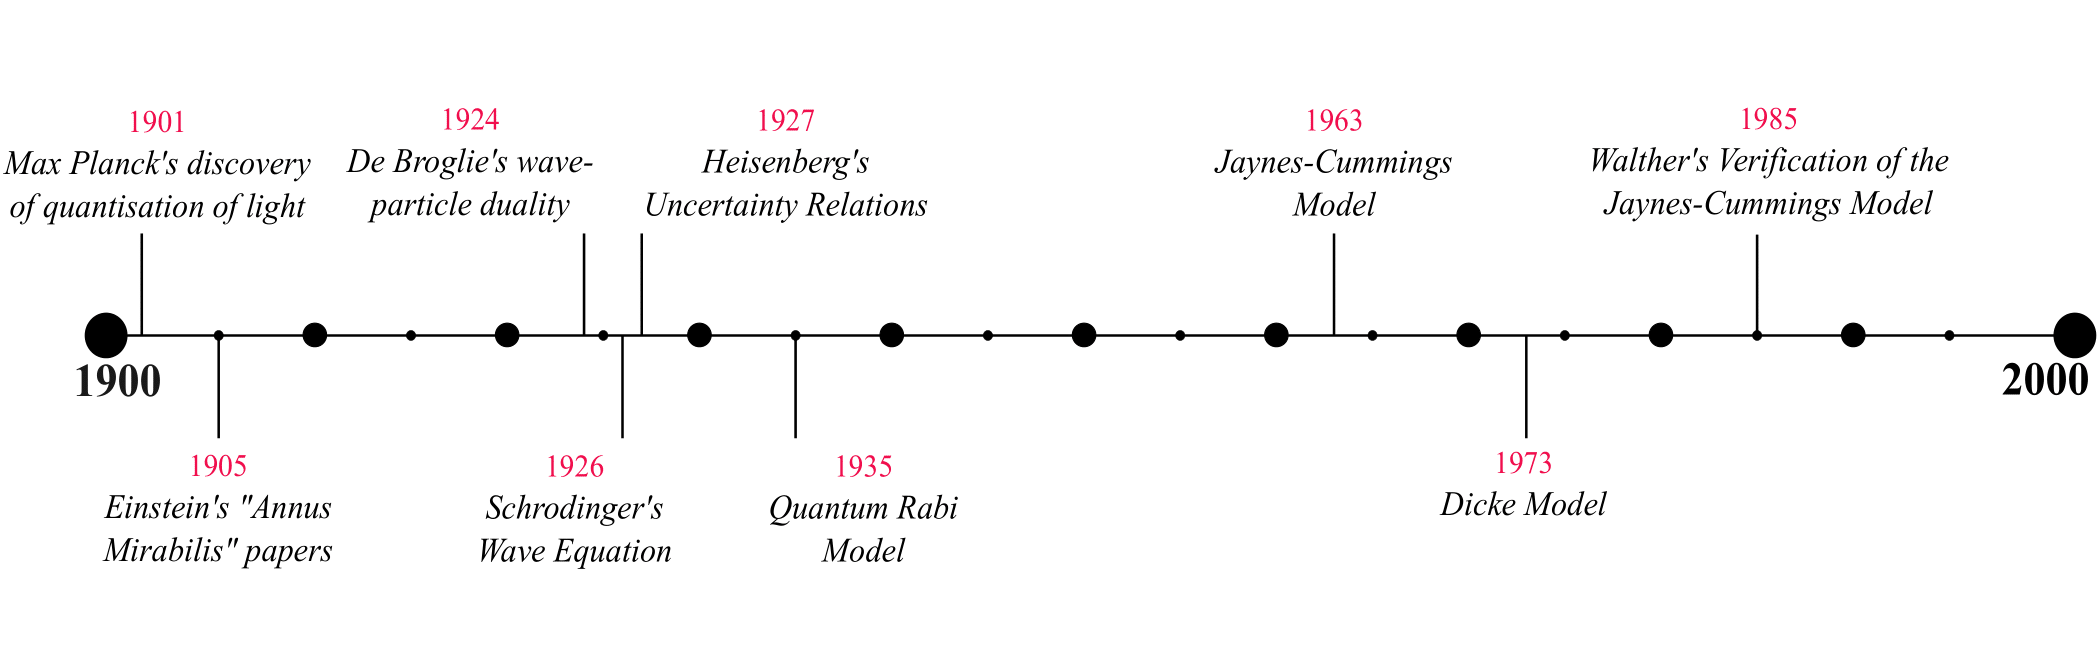
\includegraphics[scale=0.66]{timeline_JCM}
    \caption{Timeline displaying key events in both the development of Quantum Theory and quantum light-matter models.}
    \label{fig:timeline}
\end{figure}


% Rabi TLS-QHO leading to JC
Isidor Rabi was one of the first physicists to develop a theoretical framework of quantum light-matter interaction by looking at a single Two-Level System (TLS) coupled to a Quantum Harmonic Oscillator (QHO) \cite{Context1936-Rabi}. A TLS refers to any quantum system with two distinct eigenstates. In the context of the model of light-matter interaction, it refers to an atom with ground and excited energy levels. The QHO refers to a system with a harmonic potential and quantized energy levels; in this context, it refers to a quantised electromagnetic field. As we shall later discuss, Rabi's model, whilst a fairly general model of light-matter, is difficult to solve analytically and often requires computational methods. It remained one of the only reputable models of the TLS-QHO until nearly 30 years later, when in 1963 Edwin Thompson Jaynes and Fred Cummings developed the famous Jaynes-Cummings model (JCM) of the TLS-QHO while studying the field of Quantum Optics \cite{Context1963-JC_Original}. \\
% JCM and theoretical background

The two physicists set out to clarify the relationship between the quantum theory of radiation and semi-classical theory, and to apply these results to a study of the amplitude and frequency stability of a molecular beam maser (a superconducting cavity). In doing so, they produced a Hamiltonian $H$ (which describes the unitary dynamics of the TLS-QHO model, according to the Schrödinger Equation) composed of three parts \cite{Hamiltonian2012-JC_Friction}: (i) The TLS contribution $H_{TLS}$; (ii) the QHO  contribution $H_{QHO}$; and (iii) the interaction contribution $H_{int}$, which describes the coupling between the TLS and QHO. According to \cite{General2024-JCM_relevance}, the Jaynes-Cummings (JC) Hamiltonian is written as

\begin{equation}
    \hat{H} = \hat{H}_{TLS} + \hat{H}_{QHO} + \hat{H}_{int}, 
\end{equation} \label{JC_H}
where 
\begin{align*}
    \begin{aligned}
        \hat{H}_{TLS} &\equiv \frac{\hbar\omega_a}{2}\hat{\sigma}_z \\
        \hat{H}_{QHO} &\equiv \hbar\omega_ca^\dagger a \\
        \hat{H}_{int} &\equiv \hbar g(a\hat{\sigma}_{eg} + a^\dagger\hat{\sigma}_{ge}).
    \end{aligned}
\end{align*}

In equation \eqref{JC_H}, $\omega_a$ is the excitation frequency of the TLS, $\omega_c$ is excitation frequency of the QHO, $\sigma_z$ is the Pauli spin operator, $\sigma_{eg}$ and $\sigma_{ge}$ are the respective excitation and de-excitation operators that act on the TLS, $a^\dagger$ and $a$ are the respective creation and annihilation operators that act on the QHO, and $g$ is the coupling strength constant. 

One of the most striking predictions made by Jaynes and Cummings was the presence of Rabi oscillations, which is the periodic exchange of energy between the QHO and TLS, causing the TLS to oscillate between its two states, which is known as the Rabi Frequency. 

However, the technological capabilities required to experimentally verify the JCM and its predictions were not yet available. Despite this, the model garnered support from the physics community, and from the 1960s to the 1980s, theoretical work was conducted to build upon and extend the foundational framework laid by Jaynes and Cummings \cite{Context1965-TheoreticalJCM, Context1980-TheoreticalJCM, Context1984-TheoreticalJCM}. It was not until 1985 that the JCM was experimentally verified by Walther in the field of cavity Quantum Electrodynamics (cQED) \cite{Context1993-JC_Verification}. Walther injected Rydberg atoms into a maser to study non-classical radiation, mimicking the single TLS, single QHO setup of the JCM. He measured the probability of finding the Rydberg atom at the upper maser level after passing through the cavity, and found that the predictions of the JCM almost exactly matched experimental observations. Rabi oscillations were also observed.\\
\\
What began as a quantitative description of masers in Quantum Optics has now developed into a key model for understanding the intimate relationship between light and matter. Thus, from this point onwards, the JCM came to be one of the most successful models of TLS-QHO systems; its success can be attributed to its analytical simplicity and the accuracy of its predictions. This foundational model has numerous applications in a wide variety of fields, which we shall now study in detail.

\subsection{Applications} \label{JCM_apps}

One of the greatest strengths of the JCM is its simplicity. This simplicity can be attributed in part due to the Rotating Wave Approximation (RWA). The RWA neglects counter-rotating terms and primarily holds in the strong-coupling (SC) and weak-coupling (WC) regimes, thus greatly simplifying $H_{int}$ to the form shown in Equation \eqref{JC_H} \cite{General2010_USC_failure}. As a result,  the JCM finds a wide range of applications, particularly in areas where such simplifications are advantageous.

\subsubsection{Cavity QED} \label{subsubsec_cQED}

One prominent application of the JCM is in cavity quantum electrodynamics (cQED).The JCM was experimentally verified in the context of cQED, and continues to be used today to advance this field. cQED describes the interaction between atoms and the quantized electromagnetic field inside a cavity and allows physicists to gain insight into the radiative properties of the atoms \cite{General2024-JC_overview}.\\
\\
In 1995, Law and Eberly presented a cQED interaction that forced the ground state of the cavity mode to evolve into an arbitrary quantum state \cite{Context1996-CQED_JCM}. They introduced this interaction by proposing a new approach to control the quantum states of a cavity field, manipulating the quantum states of the atom during the interaction process rather than before the interaction. Notably, they modeled their system using a unitarily evolved JC Hamiltonian, and extended the model by injecting time-dependency into the coupling constant $g$ in \eqref{JC_H}.\\
\\
In 2004, Joshi and Xiao studied the non-linear transient effects of a coherent TLS entering a cavity \cite{QResJCm2004-cQED_coherence}. They found that the effects were due to the TLS in the cavity undergoing a one-photon transition in a coherent, ideal cavity field. Moreover, controlling the coherence of the atom is shown to produce two notable scenarios: (i) The outgoing atom has positive inversion for even and odd modes of the cavity; (ii) The coherent cavity is depleted owing to its mode and is dependent on the coherence of the incident atom. This study uses the exact JC Hamiltonian in \eqref{JC_H} to model the system, further highlighting the ability of the JCM to simplify complex systems while enabling fine-grain control of the quantum system. Interestingly, the authors' focus is on using coherence as a resource to modify quantum states and achieve outcomes otherwise unattainable - a subject we shall explore later in Section \ref{sec_QRes_app}.\\
\\
In 2012, Dong et al. investigated binary transmission (the process of sending information using two distinct states, typically 0 or 1) in two coupled cavities, each containing a Three-Level Atom \cite{Context2012-CQED_JCM}. They adiabatically eliminate the intermediate state of the Three-Level Atom, allowing it to be modelled by a TLS, thus enabling each TLS-QHO cavity to be described by the JCM. They explicitly mentioned that the JCM provides simple analytical solutions because the Hamiltonian is exactly diagonalizable, which enabled them to focus on the binary transmission itself. In particular, they compared the scheme using JCM analysis to one that uses the Jaynes-Cummings-Hubbard model (JCHM), a model that extends the JCM to multiple TLS and multiple mode QHOs, and facilitates the study of many-body quantum systems \cite{Context2007-JCH_1,Context2006-JCH_2,Context2006-JCH_3}. In contrast to the coupling strength $g$, if we maintain the strong coupling regime, the two-photon coupling of the JCHM $\lambda\approx0.1g$. The quantum transfer of information in the JCHM is five times slower than in the JCM due to the weaker coupling in the JCHM. On the other hand, the JCHM allows for a significantly larger propagation distance compared to the JCM, thanks to the long lifetime of metastable states. This extended distance is a result of the slower dynamics in the JCHM, which enables a more efficient transfer over longer distances. While the JCM remains a powerful tool for analysing binary transmission in cQED, the extension to multiple TLS and longer propagation distances makes the JCHM a valuable model for more complex many-body systems. This study underscores the versatility of the JCM, which, despite its limitations, continues to play a key role in advancing the study of quantum information transmission in cavity QED.\\
\\
Currently, the JCM still continues to be used in cQED, as demonstrated by recent studies exploring its applicability in modern quantum frameworks. For example, a 2024 study by Liu and Huang explored the quantum phase transition of the JCM in a cQED system \cite{Context2024-CQED_JCM}. The authors proposed a method for achieving an effective deep-strong coupling regime in a TLS coupled to a single-mode QHO. By modulating the atomic transition frequency of a TLS in a quantum Rabi model \cite{Context1936-Rabi}, they demonstrated how the effective coupling strength can be enhanced while preserving the validity of the JCM. The ability to engineer quantum phases in this setup highlights the JCM’s ongoing relevance in modern cQED research, particularly in strong and deep-strong coupling regimes. Similarly, a 2025 study by Cius investigated the unitary evolution of the JCM under fractional-time dynamics, extending its formulation using a fractional-time Schrödinger equation \cite{Context2025-CQED_JCM}. Cius highlighted how fractional calculus modifies key quantum effects in cQED, such as Rabi oscillations and atomic population inversion, while maintaining a unitary description of the system. By employing a time-dependent Dyson map, this study ensures that the JCM remains analytically solvable even in this modified framework. The study confirms that the entanglement between the atom and field is strongly dependent on the fractional-time parameter, demonstrating how the JCM continues to serve as a valuable tool in advancing our understanding of quantum coherence and cavity field interactions.

\subsubsection{Circuit QED}

Another modern, prominent field of physics that sees extensive use of the JCM is circuit QED. The TLS is modelled by a superconducting circuit that mimics artificial atoms. The QHO is modelled as a transmission line that forms a microwave cavity (see Figure \ref{fig:circuitQED}). Thus, circuit QED is analogous to cQED, instead using an artificial atom  (rather than a real atom) which is then coupled to the cavity. \\
\\

\begin{figure}[h]
    \centering
    \includegraphics[scale=1.5]{circuit_QED}
    \caption{Schematic of a superconducting circuit QED system, illustrating multiple superconducting qubits ($Q_1-Q_6$ coupled to microwave cavities. The central quantum rotor system (QRS) interacts with the qubits via tunable coupling, controlled by an external magnetic flux ($\Phi_{ext}$). Such architectures are commonly modelled using the JCM. Figure adapted from \cite{Image-CircuitQED}. Used under the terms of the CC BY license.}
    \label{fig:circuitQED}
\end{figure}

In 2004, Alexandre Blais et al. proposed the use of superconducting circuits with transmission line resonators to achieve strong coupling in circuit QED, improving qubit lifetimes \cite{Context2004-CQED_JCM}. They begin by summarising the field of cQED before proposing their methodology. The authors mentioned the JCM in their review of cQED, stating that the atomic transition frequency $\omega_1$, cavity resonance frequency $\omega_2$ and coupling strength $g$ from \eqref{JC_H} are key parameters in describing circuit QED systems. Furthermore, their Hamiltonian reduces to the JC Hamiltonian at the charge degeneracy point by neglecting both rapidly oscillating terms and damping. The paper makes it clear that the JCM's strength lies in simplifying the system, and allows us to understand the TLS-QHO interaction at its most fundamental level. \\
\\
A 2013 paper by Schmidt and Koch summarises some proposals, phenomena, and experiments that use the JCM and JCHM within circuit QED \cite{Context2013-CircuitQED}. One particular phenomenon addressed in this paper is photon blockade, a repulsion between photons inside a resonator that may be realised by a TLS-QHO model such as the JCM. The authors stated that when a weak coherent drive is in resonance with the lowest transition mode of the TLS, the cavity may only be populated by one photon owing to the photon blockade repulsion effect. This phenomenon has been experimentally observed in heterodyne transmission, resonance fluorescence spectra, and photon statistics in a linear response. The paper's conclusion reiterates a clear trend that we see throughout this review: to build an understanding of systems we need a simple model that can provide clear, reliable predictions. The JCM succeeds in providing such understanding and reliability.\\
\\
As with cQED, the JCM again finds relevant use in circuit QED. A 2024 study by Medina-Dozal et al. explored the spectral response of a non-linear JCM in the strong-dispersive regime of circuit QED \cite{Context2024-CircuitQED}. The authors extended the standard JCM by introducing non-linear deformed field operators, leading to an intensity-dependent coupling that affects the system’s spectral features. By deriving analytical expressions for the time-dependent spectral response, the study identifies asymmetries in the spectral structure that deviate from the traditional vacuum Rabi splitting. These spectral modifications provide insights into the effects of non-linearity in superconducting quantum circuits, linking the non-linear JCM to experimentally observed features in circuit QED systems. This work further reinforces the JCM as a foundational model for understanding light-matter interactions in superconducting qubits. However, the standard JCM fails to accurately describe the system in certain regimes, particularly when non-linear effects become significant, necessitating the use of a non-linear JCM. This will be further explored in Section \ref{subsec_limitations}, where we discuss how the non-linear JCM addresses these limitations in circuit QED systems.

\subsubsection{Alternative Systems}

While the JCM has proven itself as a tractable model for describing light-matter interactions in QED systems, physicists have also used it to model various other physical systems.\\
\\
One particular use of the JCM is found when looking at Nitrogen Vacancy (NV) centres, point defects in diamond lattices where a nitrogen atom replaces a carbon atom adjacent to a vacant lattice site (see Figure \ref{fig:nv_centre})\cite{General2024-JC_overview}. In a 2009 paper, Barclay et al. studied the interference phenomenon in a system where a diamond nanocrystal containing NV centres was coupled to a microdisk cavity \cite{Context2009-Alt_NVcentres}. In this case, the TLS is represented by the NV centre's single dipole transition; the QHO is the microdisk cavity. Barclay modelled the system as a cQED system and explicitly used the JC Hamiltonian to derive the density matrix equation of motion for the total system. The density matrix was then used to analyse the time evolution of the system's operators, providing detailed characterisation of the interference between the radiation emitted by the NV centre and the microdisk cavity. The JCM framework enables the calculation of optical spectra and the study of phenomena such as Fano resonances, which arise due to the interference between the direct dipole radiation and the indirect radiation mediated by the cavity mode. This approach is useful for understanding the fundamental light-matter interactions in solid-state cQED systems and highlights the potential of using NV centres in quantum information processing applications. 

The findings of this study have been used as recently as 2024 in a conference by Cheng et al. discussing the use of NV centres and GaN micro lenses to increase fluorescent light collection \cite{Context2024_NVcentre_conference}. In the same year, Bourgeois et al. released an annual review of  spectroscopy in nanoscopic cavities, where they noted that dielectric cavities, such as photonic crystals in Barclay's study, may be seen as resonators for light with high quality factors \cite{Context2024_NVcentre_review}. Bourgeois states that, because to the crystals can trap light in the cavity for long times (approximately 100 ns), they are good for controlling and modifying the electromagnetic local density of states (EMDLOS).\\
\\
\begin{figure}[h]
    \centering
    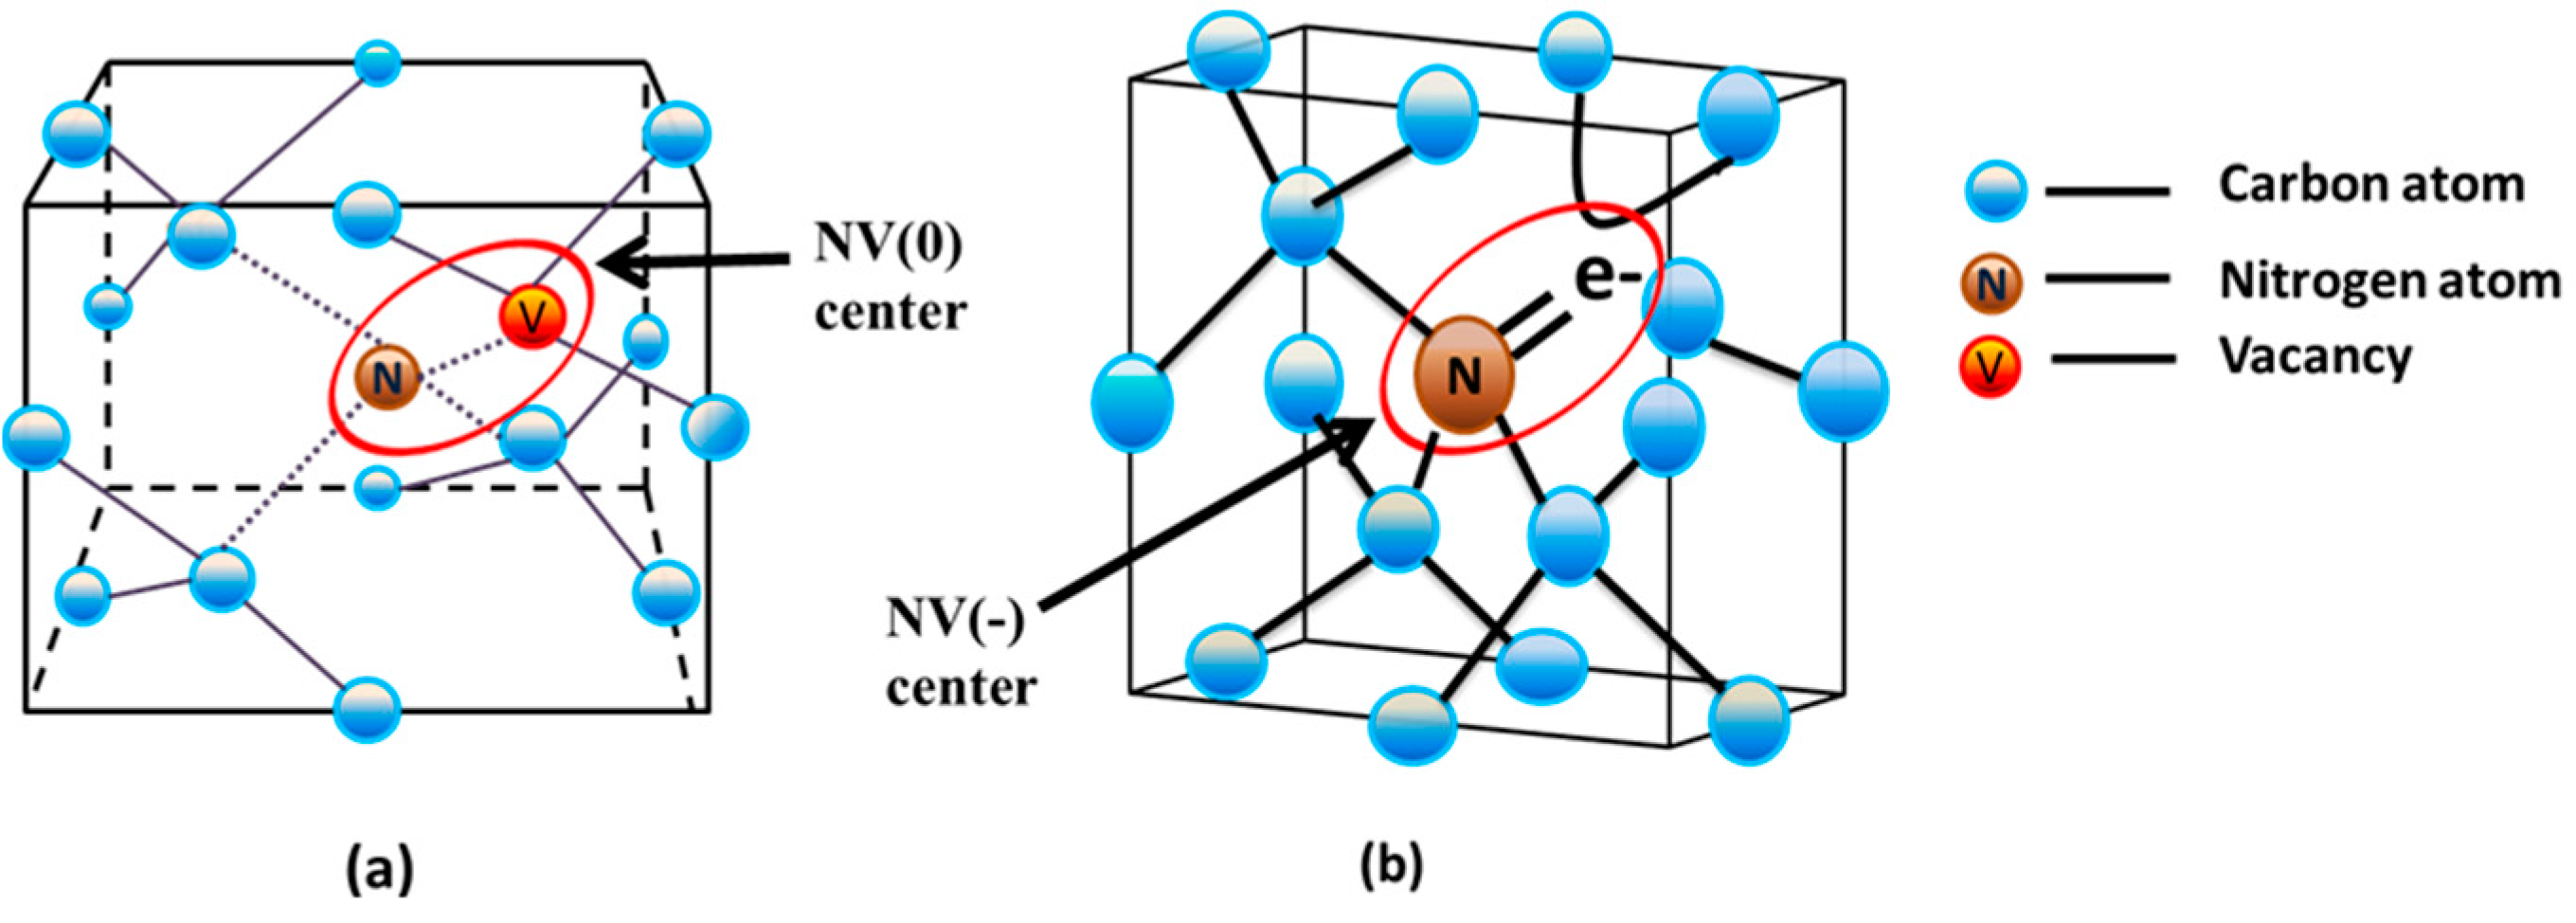
\includegraphics[scale=1.5]{nv_centre}
    \caption{Schematic of (a) NV(0) centre and (b) NV(-) centre in a diamond lattice. Figure adapted from \cite{Image-NV_centres}. Used under the terms of the CC BY license.}
    \label{fig:nv_centre}
\end{figure}

Another application of the JCM is ferromagnet-qubit systems \cite{General2024-JC_overview}. An anisotropic ferromagnet may contain magnons, which are a collection of spin excitations in magnets. When the ferromagnet is coupled to one spin qubit, the total system can be treated as a TLS-QHO. When there is no anisotropy, the JCM is sufficient for modelling the system. A 2021 study by Ida C. Skogvoll et al. demonstrates that a magnon-spin qubit ensemble can be effectively described using the JC Hamiltonian, provided that the RWA holds. In this system, a single magnon mode acts as a single-mode of a QHO, coupled with multiple spin qubits, which serve as TLSs. This study highlights a key advantage of this system: the ability to simultaneously excite multiple qubits using a single squeezed magnon mode, enabling the generation of Greenberger-Horne-Zeilinger (GHZ) states, which are crucial to quantum error correction protocols, such as Shor's error correction protocol. The protocol encodes one logical qubit into nine physical qubits, requiring entangled GHZ-like states for efficient error detection and correction. Skogvoll showed that the magnon-qubit ensemble offers a robust way to implement GHZ states, making it a strong candidate for quantum computing and quantum key distribution protocols.

However, although the JCM provides a useful approximation in this system, its validity breaks down in the presence of anisotropy. This anisotropy leads to counter-rotating terms that the JCM fails to account for under the RWA. The Quantum Rabi Model (QRM), on the other hand, includes these counter-rotating terms, and provides a more accurate description of the system dynamics. Skogvoll explicitly highlights that as anisotropy increases, deviations from the JCM become significant, requiring a transition to the QRM to fully capture the system's behaviour. This suggests that, although the JCM remains a powerful tool in many cases, its limitations become apparent in high-coupling and anisotropic regimes, a topic that will be explored in the next section.

\subsection{Limitations and Open Problems} \label{subsec_limitations}

We have seen numerous applications of the JCM within different fields of physics, and to this day, the JCM remains one of the most widely used and easily solvable models of a TLS-QHO system. However, its applicability is restricted by several inherent approximations. \\
\\
One of the main assumptions of the JCM is the simplification of a single TLS coupled to a single discrete mode of a QHO. Although this is effective in many scenarios, it fails to capture more complex interactions that arise in multi-TLS or multi-mode systems \cite{General2024-JC_overview}.

Another approximation of the JCM is the RWA. As previously discussed in Section \ref{sec_TLS-QHO}, the RWA neglects counter-rotating terms and holds primarily in the SC and WC regimes. For example, in the context of cQED, the RWA is:

\begin{equation}
    \boldsymbol{\hat{d}}\cdot\boldsymbol{\hat{E}} \propto (\hat{\sigma}_{eg} + \hat{\sigma}_{ge})(a + a^\dagger)\approx (a\hat{\sigma}_{eg} + a^\dagger\hat{\sigma}_{ge}), \label{RWA}
\end{equation}

where $\boldsymbol{\hat{d}}$ is the dipole moment operator associated with the TLS, and $\boldsymbol{\hat{E}}$ is the electric field operator associated with the QHO \cite{General2024-JCM_relevance}. Several papers \cite{General2010_USC_failure, Context2024-CircuitQED} addressed these issues by using the non-linear JCM, an extension of the original model. 
We shall now explore the failures of the JCM in certain coupling regimes, and alternative models that compensate for these pitfalls.

\subsubsection{Coupling Regimes and the Breakdown of The Jaynes-Cummings Model}

In the WC regime, the coupling strength satisfies $g \ll \kappa, \gamma$, where $\gamma$ represents the decay rate of the TLS and $\kappa$ is the decay rate of the QHO \cite{Context2017-USC_failure}. In this regime, dissipative processes dominate, and energy exchanged between the TLS and the QHO is rapidly lost to the environment, preventing coherent oscillations from developing. As the coupling strength increases beyond the loss rates, the system enters the SC regime, which is characterized by $g > \kappa, \gamma$. Here, coherent interactions prevail, allowing the TLS and the QHO to exchange energy multiple times before decoherence occurs.

The JCM provides an accurate description of this regime, successfully predicting Rabi oscillations, which are periodic energy exchanges between the TLS and the QHO \cite{Context1993-JC_Verification}. This process causes the TLS to transition repeatedly between its ground and excited states, oscillating at the Rabi frequency $\Omega_R$ \cite{Context_-Rabi_oscillations}. These oscillations are a hallmark of strong coupling and serve as experimental signatures of coherent light–matter interaction.

In a 2024 review of the JCM, De Bernardis et al. examined the continued relevance of the JCM in modern cavity QED and discussed the various approximations that underpin its validity \cite{General2024-JCM_relevance}. Bernardis states that in the SC regime, $\Omega_R > \kappa, \gamma$, and defines the cooperativity parameter as $C = 4\Omega^{2}_R/(\gamma\kappa)$, and $C > 1$ marks the SC regime. Furthermore, $\Omega_R > \omega_c, \omega_a$, where $\omega_c, \omega_a$ are the bare excitation frequencies of the QHO and TLS respectively (see Equation \eqref{JC_H}). However, in the ultrastrong-coupling (USC) regime, the coupling strength is no longer a small perturbation but becomes comparable to the bare excitation frequencies. Bernardis introduces an analogy to the cooperativity parameter, defining the normalised coupling parameter as $\zeta = 4\Omega^{2}_R/(\omega_c\omega_a)$, where $\zeta \sim \mathcal{O}(1) $ indicates the USC regime. Importantly, Bernardis emphasises that the cooperativity parameter is not sufficient to describe the USC regime. In certain experimental systems such as Rydberg atoms in cavities, the cooperativity parameter is much greater than $1$ ($C \sim 10-100$), and the normalised coupling parameter remains small ($\zeta \sim 10^{-5} $), yet the JCM still remains applicable. However, in other experiments such as superconducting qubits in cavities, $\zeta \gg 1$, a regime in which the JCM is not valid. Thus, $C$ does not indicate when the coupling strength is large enough to invalidate the JCM’s structure. Instead, $\zeta$ serves as an appropriate measure to distinguish systems in which the JCM remains valid.\\

\begin{table}[h]
    \centering
    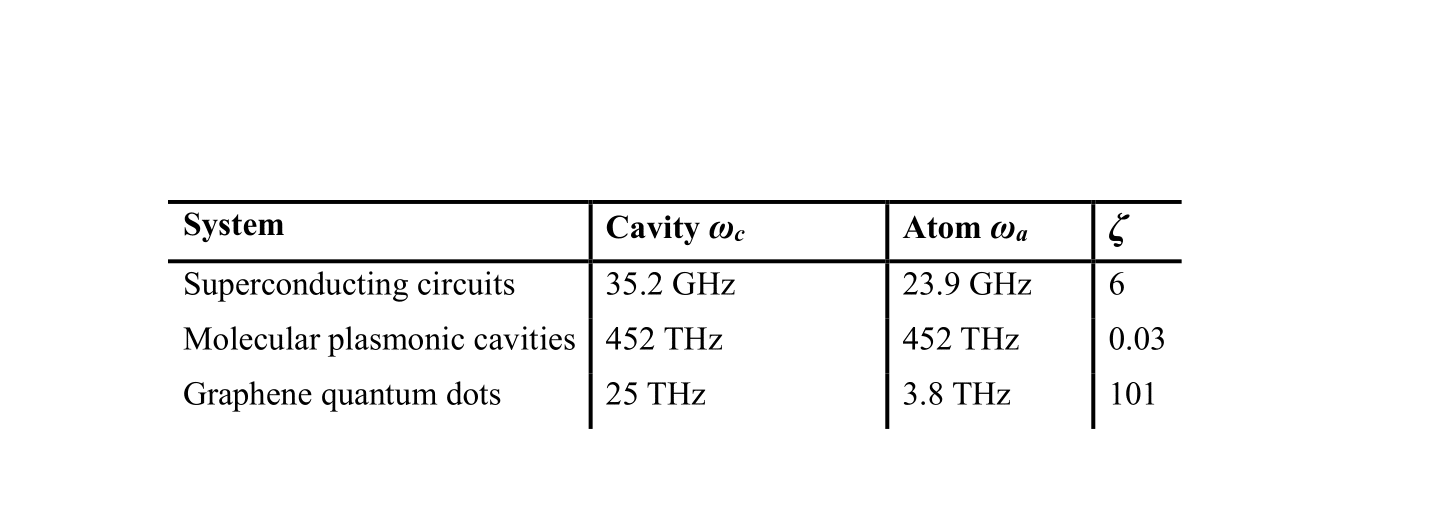
\includegraphics[scale=1]{coupling_strengths}
    \caption{Parameters of various cQED setups in which the TLS-QHO system reaches the USC regime. The table shows that for certain experimental set-ups, including superconducting circuits and molecular plasmonic cavities,  $\zeta \sim \mathcal{O}(1) $ and the JCM may still hold. However, for $\zeta \gg 1$, the JCM fails. See references [25-27] in \cite{General2024-JCM_relevance} for data.}
    \label{fig:nv_centre}
\end{table}


The failure of the JCM is not solely due to the large coupling strength relative to the system’s fundamental frequencies (quantified by $\zeta$), but also because of one of the key approximations of the JCM: the RWA \cite{General2024-JCM_relevance}. In the same 2024 review, Bernardis also examined the breakdown of the RWA in the USC regime. The RWA neglects counter-rotating terms (see equation \eqref{RWA}) which in turn describe processes where a photon may simultaneously be created/annihilated with a respective excitation/de-excitation of the TLS. In the WC and SC regimes, these counter-rotating terms are considered negligible and commute with the excitation number operator $|n\rangle$ of the QHO. This commutation gives the JCM a $U(1)$ symmetry; the JCM can thus be expressed in a block-diagonal form, which in turn provides a simple analytical solution. However, in the USC regime, the coupling strength is comparable to the bare excitation frequencies, and the counter-rotating terms can no longer be neglected. The counter-rotating terms no longer commute with  $|n\rangle$, and the $U(1)$ symmetry is broken. The JCM no longer has a simple analytical solution, and new interactions emerge, whose effects are not captured by the JCM. 

One of the clearest experimental observations of the RWA breakdown is the Bloch-Siegert shift. If the driving force of a QHO is strong enough that the Rabi frequency approaches the Larmor Frequency ($\omega_a/2\pi$), the counter-rotating terms are non-negligible. This leads to a shift in the energy-level transition of the TLS, known as the Bloch-Siegert shift \cite{Context2010-Bloch_Siegert}. In 2010, Forn-D\'iaz et al. experimentally observed the Bloch-Siegert shift when studying a resonant circuit (modelled as a QHO) coupled to a superconducting qubit (modelled as a TLS). The system's interaction strength reaches $g/\omega_c \approx 0.1$, which is in the USC regime. Forn-D\'iaz observes a 50MHz energy shift in the qubit's energy-level transition, verifying the Bloch-Siegert shift and demonstrating the RWA's breakdown in USC regimes. Moreover, Forn-D\'iaz compared the experimental results to the JCM and the Quantum Rabi Model, and concluded that the Rabi Model accurately describes the experimental results, whereas the JCM's predictions fail. This experimental validation of the Bloch-Siegert shift reinforces the need for more general models beyond the JCM, such as the Quantum Rabi Model and the Dicke Model, which fully account for non-perturbative light–matter interactions.


\subsubsection{Alternative Models}

One of the primary alternatives to the JCM in the context of a single TLS coupled to a single quantised mode of a QHO is the Quantum Rabi Model (QRM) \cite{Context1936-Rabi}. As outlined in Section \ref{subsec_history}, the QRM was formulated in 1936, nearly 30 years before the JCM. However, the drawback to the model is that it is not exactly solvable \cite{Hamiltonian2017-Rabi}. The JCM was therefore devised as a model that sought to simplify the QRM by applying the RWA. According to \cite{General2024-JCM_relevance}, the QRM can be described by the Hamiltonian

\begin{equation}
    \hat{H_R} = \hat{H}_{TLS} + \hat{H}_{QHO} + \hat{H}_{int}, 
\end{equation} \label{JC_H}
where 
\begin{align*}
    \begin{aligned}
        \hat{H}_{TLS} &\equiv \frac{\hbar\omega_a}{2}\hat{\sigma}_z \\
        \hat{H}_{QHO} &\equiv \hbar\omega_ca^\dagger a \\
        \hat{H}_{int} &\equiv \hbar g(a + a^\dagger)\hat{\sigma}_{x},
    \end{aligned}
\end{align*}

where $\hat{\sigma}_{x}$ is the Pauli matrix for the TLS. The difference between the Rabi and JC Hamiltonians is the interaction part of the Hamiltonian $H_{int}$. For the QRM, the interaction Hamiltonian can be written as the sum of two terms:
$\hbar g(a + a^\dagger)\hat{\sigma}_{x} = g(\hat{\sigma}_{ge}a^\dagger+\hat{\sigma}_{ge}a) + g(\hat{\sigma}_{ge}a^+\hat{\sigma}_{ge}a^\dagger)$ \cite{Hamiltonian2017-Rabi}. This decomposition directly displays the rotating and counter-rotating terms as seen outside the RWA approximation. Thus the QRM has a clear advantage over the JCM: if we consider systems in which the RWA is invalid, the QRM can fully capture the system in its description. On the one hand, the QRM has no simple analytical solution. This is because the QRM's counter-rotating term does not commute with the excitation number operator, and the $U(1)$ symmetry is not present. On the other hand, the QRM is still numerically diagonalisable, with libraries such as the QuTip Python library providing the necessary methods \cite{General2024-JCM_relevance}. 
The QRM, when the coupling is small, is indistinguishable from the JCM. In higher-strength coupling regimes, such as the USC, we find that the difference between the two models becomes greater due to the counter-rotating terms are more prominent \cite{General2024-JCM_relevance}. A consequence of these counter-rotating terms is that the empty cavity vacuum (i.e., the ground state) is no longer an eigenstate of the system, and we find virtual photons present in the coupled ground state of the system itself. In fact, one of the central ideas in the development of cQED in the USC regime was to detect these virtual photons. It is clear that the main advantage of the QRM is in fully capturing system dynamics in the USC and beyond, where counter-rotating terms become increasingly prominent. In using the QRM, however, we lose intuition and simple analytical solvability.\\
\\
Another alternative to the JCM is the Dicke model \cite{Context1954-Dicke}. In 1953, Robert Dicke introduced the Dicke Model to describe superradiance by considering light emission from a large ensemble of atoms (modelled as an ensemble of TLS's) coupled to a single quantised mode of a cavity (modelled as a QHO) \cite{Hamiltonian2019-Dicke}. The corresponding Dicke Hamiltonian is written as 

\begin{equation}
    \hat{H}_D = \omega_ca^\dagger a  +\omega_a\sum^N_{j=1}\hat{\sigma}_j^z + \frac{2\lambda}{\sqrt{N}}(a + a^\dagger)\sum_j\hat{\sigma}_j^x,
\end{equation}

where $\hat{\sigma}_j^z$ and $\sigma_j^x$ are the Pauli spin operators, N is the number of atoms in the ensemble, and $\lambda$ is the TLS-QHO coupling strength \cite{Hamiltonian2019-Dicke}. Unlike both the JCM and QRM, the Dicke model accounts for an ensemble of TLS's in a QHO environment, which collectively enhances the Rabi frequency by a factor $\sqrt{N}$. This ensemble of TLS's allows a system that utilises the Dicke model to achieve USC regimes far more easily than that of the single TLS setups of the QRM and JCM. One of the most striking consequences of this model is the emergence of superradiance, a phase transition where the TLS ensemble spontaneously emits photons, which is absent in the JCM and QRM. Furthermore, the Dicke model is exactly solvable in the thermodynamic limit ($ N \rightarrow \infty$), because the system is better described by a linear optical approach where the cavity and material may both be described by QHOs \cite{General2024-JCM_relevance}. However, it is not clear what this linearity has on modifying ground-state properties. Furthermore, it has been shown that many other single-particle effects are not enhanced by the ensemble of TLSs; in fact the Dicke model makes it harder to modify the properties of matter in the system. Thus, the Dicke model extends the JCM and QRM to an ensemble of TLSs, making it an ideal framework for studying quantum many-body effects in cQED. However, the ensemble does not necessarily enhance many desirable effects, and the only notable effect is the enhancement of the Rabi frequency. Given the more complex nature of the Dicke model, it is generally even more difficult to solve than the QRM, making the model undesirable for use in a single TLS-QHO system, where the QRM and JCM are favoured. \\
\\
It is clear that even to this day the JCM prevails as one of the simplest models of a TLS-QHO, especially in the context of describing quantum light-matter systems. However, the model has certain limitations, such as its failure to correctly capture a system dynamics in stronger coupling regimes. Nevertheless, its strength lies in its ability to produce clear, reliable predictions. A key aspect of modelling a system (and one that is inevitable) is the approximations, and by starting with the simplest possible description, such as the JCM in light-matter system, we can progressively introduce complexity through extending the model itself. While other models such as the QRM and Dicke Model have certain advantages (such as being valid in stronger coupling regimes, or describing collective effects of an ensemble of TLSs), the JCM still remains a clear, exactly solvable, and intuitive model that physicists will undoubtedly continue to use to understand system dynamics. Beyond system dynamics, however, modern quantum technologies and systems increasingly rely on quantum resources such as entanglement and coherence, to access, control and manipulate quantum states. Understanding how these resources emerge and evolve is essential for advancing theoretical and experimental studies. We now explore these fundamental quantum properties and examine their current use within the scope of the JCM.


\section{Quantum Resources: Entanglement and Coherence} \label{sec_QRes}

Quantum resources form the foundation of quantum information science, enabling quantum technologies such as computation, communication and key distribution. Among the various resource theories, entanglement and coherence are two of the most fundamental and widely studied \cite{CohEnt2019-QRT_def}. Entanglement identifies the separability of a quantum state, whereas coherence captures the degree of superposition in a quantum state. Although entanglement has long been regarded as the primary quantum resource, coherence, a relatively new resource, is gaining significant traction \cite{CohEnt2019-QRT_def}. This section explores formal definitions and various key measures of both entanglement and coherence. 

\subsection{Entanglement} \label{subsec_ent}

The most distinguished quantum resource is entanglement, a unique quantum phenomenon that describes non-classical correlations between subsystems of a composite quantum system. A total state $|\Psi\rangle$ is said to be entangled if it cannot be written as a product state, that is:

\begin{equation}
    |\Psi\rangle \neq |\psi_A\rangle \otimes |\psi_B\rangle,
\end{equation}

where $|\psi_A\rangle, |\psi_B\rangle$ are the pure states of subsystems A and B respectively. If a state \textit{can} be expressed in this form, it is considered separable and exhibits only classical correlations. The quantification of pure state entanglement has been rigorously examined, and measures such as Von Neumann Entropy (VNE) suffice. However, mixed state entanglement quantification is significantly more challenging. \\
\\
One of the most celebrated measures of Entanglement is the VNE. Petz neatly summarised Johann von Neumann's seminal measure of Quantum Entanglement in a 2001 paper \cite{Entanglement2001-VNE_Definition}. Von Neumann's entropy measure generalises the classical Shannon entropy to quantum systems by quantifying the extent to which a state is mixed (and by extension, entangled). Petz highlights that von Neumann derived his formulation of entropy in a 'gedanken' (thought) experiment in his search for a formalism of quantum thermodynamics. Von Neumann showed that quantum entropy behaves analogously to its classical counterpart while incorporating unique quantum features. Mathematically, the VNE \cite{Entanglement2001-VNE_Definition} measures the degree of entanglement for a pure bipartite system $|\Psi\rangle$(such as the TLS-QHO system), and depends on either of the subsystem density matrices' eigenvalues:

\begin{equation}
    S_{vn}(\rho) = -\text{Tr}(\rho\log({\rho})),
\end{equation}

where $\rho$ is the density operator of the bipartite system. Petz further highlighted that the entropy of a subsystem $\rho_{sub}$ of $\rho$ also fully captures the entanglement of the total state if the density operator of the total state is pure. If the subsystems are entangled, then $S(\rho_{sub}) > 0$, whereas if they are separable, then $S(\rho_{sub}) = 0$. Petz also noted the mixing property of entropy, showing that the VNE increases under quantum measurements, reflecting the irreversibility of quantum states. The VNE finds itself at the forefront of Entanglement quantification, and is a canonical measurement of entanglement itself. In 2019, Lent examined the entropy of pure state operators under unitary evolution, and found that under unitary evolution, the state is completely reversible with no loss of quantum information \cite{Entanglement2019_VNE_example}. Moreover, he verified that entropy increases in a way that is analogous and consistent to classical statistical entropy and the second law of thermodynamics. We find another use of the VNE as recently as Febuary 2025, wherein Ram Narayan Deb provided a generalised relationship between the VNE of the subsystems of a composite state, and different types of squeezing in the context of Ramsey spectroscopy \cite{Entanglement2025_VNE_example}. In Section \ref{sec_QRes_app}, we discuss further applications of the VNE in the context of a TLS-QHO system. \\
\\
The Relative Entropy of Entanglement (REE), as formulated by Vedral and Henderson in 2000, provides a more general framework for quantifying entanglement, particularly for mixed states \cite{Entanglement2000-REE_definition}. The REE is defined as: 

\begin{equation}
    E_{REE}(\rho) = \min_{\sigma \in D}  S(\rho||\sigma),
\end{equation}

where $ S(\rho||\sigma) = \text{Tr}(\rho\log(\rho) - \rho\log(\sigma))$ is the quantum relative entropy, and the minimisation is performed over the set $D$ of all separable states $\sigma$. This formulation quantifies the 'distance' between an entangled state and the closest separable state. 

Vedral and Henderson showed that REE serves as an upper bound on distillable entanglement, which is the amount of pure entanglement extractable from a mixed state using local operations and classical communication (LOCC). They further mentioned that other entanglement measures, such as the Entanglement of Formation (EoF) and the VNE, may be seen as special cases of REE, thus establishing the measure as a unification of other entanglement measures. A key result of the authors' work is the irreversibility of entanglement transformation in mixed states. Unlike pure states, where entanglement can be converted between different forms, mixed-state entanglement exhibits asymmetry, and the entanglement required to create a mixed state (EoF) is always greater than distillable entanglement. This discrepancy arises due to the loss of classical information about the state, and is a feature that the REE captures explicitly. Compared to the VNE, the REE is more general, as it applies to both pure and mixed states and applies entanglement beyond well-defined bipartite systems. The REE for mixed states, however, is notoriously difficult to calculate analytically, and requires numerical methods to compute \cite{Entanglement2009-REE_VNapplied}, unlike the VNE, which has an incredibly simple analytical solution. \\
\\
While the VNE and REE are key measures for pure and mixed states respectively, there are other notable measures of entanglement that we shall now briefly explore. 

Wootters introduced concurrence as a measure of entanglement specifically for a pair of qubits, providing a direct method for computing the EoF for mixed states \cite{Entanglement2001-WC_qubits}. The concurrence, $C(\rho)$ of a pure two-qubit density matrix is given by $C(|\Psi\rangle) = |\langle\psi|\Tilde{\psi}\rangle|$, where $|\Tilde{\psi}\rangle = (\sigma_y\otimes\sigma_y)|\psi*\rangle$ is the spin flipped state of $|\psi\rangle$. Wootters established the connection between concurrence and EoF by showing that, for a two-qubit system, the EoF is given by

\begin{equation}
    E_f(\rho) = h\left(\frac{1+\sqrt{1-C^2}}{2}\right),
\end{equation} 

where $h(x) = - x\log_2x - (1 - x)\log_2(1 -x)$ is a binary entropy function. The significance of concurrence is in providing an exact formulation of the EoF, which was until then difficult to compute for mixed states. Compared to the REE, concurrence offers a simple approach to entanglement quantification for mixed-state entanglement, but is limited in its scope to two-qubit systems. Efforts have been made to expand concurrence to arbitrary dimensions \cite{Entanglement2001-WC_arbdim}, with some success in qudit (d-dimensional qudit) systems as recently as 2025 \cite{Entanglement2025_WC_arbidm_example}. However, this measure is not yet applicable to single TLSs coupled to one quantised mode of a QHO.

Another well-known measure of entanglement is the Entanglement R\'enyi $\alpha$-entropy (ER$\alpha$E). In 2016, Wang et al. discussed ER$\alpha$E, noting that the measure introduced a continuos parameter $\alpha$ to the VNE, thus providing a broader spectrum of entanglement measures \cite{Entanglement2016-ERaE_Definition}. The ER$\alpha$E, for a pure state $|\Psi\rangle$ with subsystems A and B, is defined as

\begin{equation}
    R_{\alpha}(|\Psi\rangle) \equiv \frac{1}{1-\alpha}\log_2{\text{Tr}(\rho_B^\alpha)},
\end{equation}

where $\rho_B^\alpha$ is the subsystem of the reduced density operator of the total state $|\Psi\rangle$. Wang stated that for pure bipartite states the ER$\alpha$E reduces to the VNE in the limit $\alpha \rightarrow 1$, yet again showing the importance of the VNE as a specialised measure of entanglement for pure states. The generalisation to mixed states follows a convex-roof construction method, which in turn requires a minimisation over all possible pure state decompositions, making the calculation computationally difficult. Compared to the previous entanglement measures, the ER$\alpha$E uniquely presents a continuos measure of entanglement over the spectrum of $\alpha$, enabling finer-grain tuning of the entanglement measure. This makes the ER$\alpha$E particularly useful in contexts where we want to capture more nuanced details in the entanglement structure of the system. 

\subsection{Coherence}

Although entanglement remains the most studied and used quantum resource, another fundamental phenomenon that has gained traction is coherence. Streltsov et al. extensively reviewed coherence in a 2017 colloquium, defining the resource as the ability of a quantum state to exhibit superpositions in given basis of choice \cite{Coherence2017-Colloquium}. Streltsov stated that, while coherence has been experimentally studied in optical physics, its role as a quantum resource has only recently been formalised within the axiomatic theoretical framework of Quantum Resource Theory as described in \cite{CohEnt2019-QRT_def}. Despite its major role in quantum computation and quantum thermodynamics, coherence is a rapidly evolving field of quantum physics. \\
\\
A key measure of coherence is the Relative Entropy of Coherence (REC) \cite{Coherence2014-seed}. In 2014, Baumgratz et al. the introduced general distance-based coherence measure:

\begin{equation}
    C_D(\rho) = \inf_{\sigma \in I} D(\rho,\sigma),
\end{equation}

where D is the distance and we take the infimum over the set of incoherent states, and $\sigma$ is the reference state. If, similar to entanglement, we take the distance measure to be the quantum relative entropy, we obtain the REC, $C_r$:

\begin{equation}
    C_r(\rho) = C_d(\rho) = S(\rho_{diag}) - S(\rho),
\end{equation}

where $S$ is the VNE, and $\rho_{diag}$ is the state obtained by removing all off-diagonal elements. From this formalism Baumgratz noted one of the defining features of coherence: basis dependency. For any composite system, the preferred basis for studying coherence is the tensor product of the corresponding local reference basis state for each subsystem. Furthermore, the REC aligns closely with the quantum relative entropy measure used in entanglement theory. In fact, its formulation mirrors the REE, where coherence plays the role of quantifying quantum correlations. This connection reinforces the role of coherence as a fundamental quantum resource, analogous to entanglement. A 2024 paper by Lecamwasam et al. examined the REC as a quantifier of performance in Bayesian metrology \cite{Coherence2024-REC_development}. In particular, Lecamwasam showed that REC can be applied to an ensemble of states, and noted that the REC of the ensemble allows visualisation of the amount of information that is inaccessible within a given measurement scheme applied to a system. \\
\\
Another important measure of coherence is the coherence norm. In the same 2014 paper which defined the REC, Baumgratz defined the norm, $C_l$, as a direct measure of a state's off-diagonal elements \cite{Coherence2014-seed}:

\begin{equation}
    C_l(\rho) = \sum_{i,j}|\rho_{i,j}|.
\end{equation}

Similar to the REC, the norm is a computationally accessible measure of coherence. However, Baumgratz states that unlike the REC, the norm lacks a clear interpretation in terms of coherence distillation. Another distinction from the REC is that the norm is highly sensitive to small coherence contributions, making it a valuable tool for detecting weak coherence in quantum systems. However, the sensitivity of this measure can lead to challenges in experimental implementation, where small fluctuations can significantly change the measured coherence. Similar to the REC, the coherence norm is still being develope. In a 2024 paper by Yang et. al., the coherence norm's formalism is refined with tighter superadditivity inequalities and extended to arbitrary multi-qubit states \cite{Coherence2024-Norm_refinement}.

Now that we have defined quantum resources and explored the key measures of entanglement and coherence, it is important to examine their role in the JCM.


\section{Application of Quantum Resources to The Jaynes-Cummings Model} \label{sec_QRes_app}

As discussed in Section \ref{sec_TLS-QHO}, the JCM can capture many physical systems in its description. Quantum resources, however, have recently become of great interest to physicists studying quantum systems because they provide insight into system dynamics and allow fine-grain control over quantum states. Thus, investigating these resources within the JCM is essential for unlocking the model's full potential and aligning with current advancements in quantum information science. In this section, we explore how entanglement and coherence measures can be applied within the JCM to characterise systems and develop experimental control mechanisms. \\
\\
As previously mentioned in \ref{subsubsec_cQED} in the context of cQED, in \cite{QResJCm2004-cQED_coherence}the authors stated that controlling the coherence of the atom (TLS) directly influences how quickly the cavity (QHO) is depleted. This study hints at manipulating coherence in the TLS to control the lifespan of the cavity. This is exactly what Messinger expanded on later in a 2020 paper, in which she explored coherence in the JCM by examining how TLS-modelled atoms (individually fed into the cavity) interact with a QHO-modelled cavity \cite{CohEnt2020-Cavity_controlled_coherence}. This study builds upon the exact JC Hamiltonian in Equation \eqref{JC_H}. Messinger focused on coherence transfer from the cavity to the atoms, and analysed the degradation of coherence in the cavity as it is distributed among atoms, quantifying coherence using the REC. Her key finding is that the initial coherence in the cavity is not immediately depleted; rather, there is an enhancement in the coherence up to an optimal number of atom-cavity interactions. Specifically, the cavity can be used for approximately $\mathcal{O}(n^2)$ atomic interactions before degradation becomes significant. This phenomenon is related to the JCM's ability to preserve the total excitation number. Furthermore, she tied her study to coherence catalysis, which is the ability to repeatedly extract coherence without degradation. By using the JCM as a tool to achieve simple, intuitive analytical results, this study highlights the practical implications of coherence control in cQED.\\

\begin{figure}[h]
    \centering
    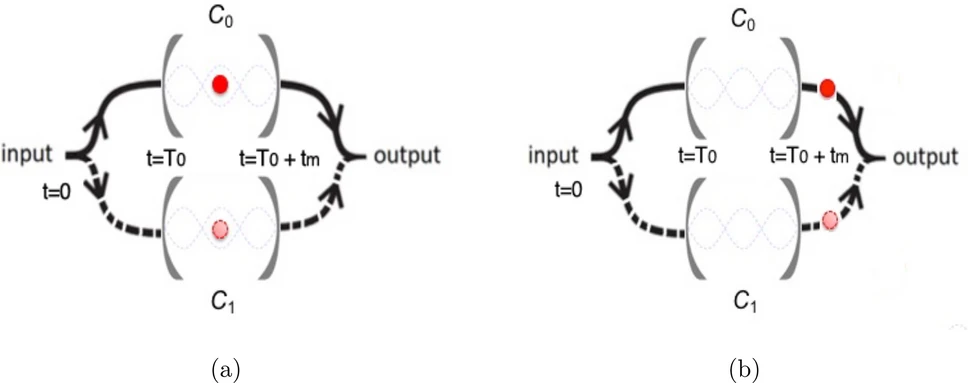
\includegraphics[scale=0.3754]{coh_ent_2x_cavity}
    \caption{Schematic of an atom entering the cavities. Depending on the preparation of the atom, which in turn is controlled by the control qubit, the atom interacts with only one of the two cavities $C_0, C_1$ at a time. (a) The atom enters at a time $t = T_0$ after preparation, and (b) exits at $t = T_0 + t_m$ to the output. Figure adapted \cite{CohEnt2024-2_JCM_coherence}. Used under the terms of the CC BY 4.0 license.}
    \label{fig:double_cavity}
\end{figure}

A recent 2024 study by Castaños-Cervantes et al. continues the exploration of coherence in the JCM by examining single atoms streamed into one of two separate single-mode cavities  \cite{CohEnt2024-2_JCM_coherence}. As in \cite{CohEnt2020-Cavity_controlled_coherence}, the Hamiltonian in equation \eqref{JC_H} is used to describe the system. Coherent control of the two cavities in this system is said to enable novel possibilities of atomic manipulation, which was not previously possible. Castaños-Cervantes first defined a control qubit that determines the cavity that the atom interacts with. If the qubit is in the basis state $|0\rangle$, the atom interacts with the $C_0$ cavity. If the qubit is in the basis state $|1\rangle$, the atom interacts with the $C_1$ cavity. By preparing the qubit in a superposition state, the atom interacts with both cavities simultaneously, introducing coherence between the two modes as follows:

\begin{equation}
    |\theta,\phi\rangle_c = \cos{\theta}|0\rangle_c + e^{i\phi}\sin{\theta}|1\rangle_c,
\end{equation}

where $\theta$ controls the weight of the superposition between the basis states of the qubit and $\phi$ represents the phase factor between the two basis states. The study then explores how this coherence affects the atomic population inversion, and finds that controlling the coherence of the atom-cavity interaction yields a tunable Rabi frequency and enables control of quantum state preparation. Moreover, Castaños-Cervantes demonstrated that coherence in the JCM can be used to generate entangled states of the cavity by measuring the qubit and atom after the interaction. This study extends the JCM into modern quantum information science by using coherence to control the system in novel ways. Furthermore, it touches on entanglement within the model, which we shall now examine.\\
\\
In a 2009 paper, Hern\'andez Concepci\'on et al. examined entanglement in a continuously measured TLS coupled to a QHO, again using the JC Hamiltonian in equation \eqref{JC_H} to model the system and extend it to include the measurement effects \cite{Entanglement2009-REE_VNapplied}. Entanglement is quantified using two key measures: the VNE and REE, using the same formulations as in Section \ref{subsec_ent}. The study finds that, due to the 'flip-flop' effect of the TLS-QHO interaction, the VNE oscillates between 0 and $\ln{2}$. The study then numerically computes the REE and finds that a double peak structure emerges in the REE distribution, indicating that entanglement is maximised at a coupling strength $g\approx0.5$ and a QHO decay rate of $k\approx1$ both expressed in units of the TLS decay rate $\gamma$. Overall, the study found that entanglement persists despite the degradation of the system to the environment. 

%%%%%^% INSERT IMG OF ABOVE STUDYy

Larson et al. provide a comprehensive summary of the JCM in a 2024 book \cite{General2024-JC_overview}. Larson discussed entanglement as a key quantum resource that emerges within the TLS-QHO system. It reviews historical contributions and examines the first introduction of entanglement in the JCM in the 1990s, using the VNE measure. Since the JCM preserves the total excitation number, measuring the three components of the Bloch vector of the JCM allows direct access to entanglement. The study also employed concurrence as a measure of the bipartite entanglement of the JCM, computing the concurrence using the eigenvalues of the spin-flipped density matrix of the system. Larson found that the concurrence exhibits oscillatory behaviour within two-TLS JCM systems. This mirrors the VNE calculations of \cite{Entanglement2009-REE_VNapplied}, albeit with a maximum concurrence of $C_{max}\approx0.98$, indicating near-maximal entanglement between the TLS and QHO (because concurrence ranges from 0 to 1). Larson also highlighted the dependence of entanglement on the initial state. As in \cite{Entanglement2009-REE_VNapplied}, if the atom starts in an excited state, entanglement grows significantly over time. Overall, the JCM is shown to be a fundamental model for studying entanglement in quantum light-matter interactions, and enables control of a quantum state through initial conditions. 

\section{Conclusion} \label{sec_Conclusion}

The JCM is a canonical model for quantum light-matter interaction. In this review, we have highlighted a range of systems which the JCM fully and accurately captures in its descriptions, from well-established fields like cQED, to emerging, nascent fields such as NV centres and circuit QED. However, the JCM has limitations: it breaks down in the USC regime due to the failure of the RWA, and does not account for multi-TLS multi-QHO coupling. In such cases, the Rabi Model and Dicke model provide more appropriate descriptions. The trade-off, however, is that these models usually require complex (and often numerical) analyses, whereas the JCM provides intuitive, simple analytical solutions. Due to this, the JCM is ideal for focussing on systems where there is only one TLS interacting with one quantised mode of a QHO up to the SC regime. Furthermore, the model provides simple, reliable predictions while allowing for increased complexity through extensions.\\
\\
Beyond its role in describing physical interactions, the JCM provides a simple and intuitive framework for extracting quantum resources such as entanglement and coherence. The primary entanglement measures considered in recent studies are the VNE and the more computationally intensive REE. The R\'enyi entanglement entropy measure has not been thoroughly explored within the JCM and remains an open problem. Studies of entanglement in the JCM have revealed oscillatory behaviour in systems like the two-TLS JCM, where concurrence exhibits near-maximal entanglement when the TLS is initially excited. Using the R\'enyi entanglement in such scenarios could offer a promising way to explore the observed oscillatory behaviour in such systems, due to its tunable $\alpha$ parameter which finer control over entanglement quantification.

For coherence, the REC has been the primary measure, with studies demonstrating that controlling the TLS's coherence enables control over the cavity. However, the coherence norm remains relatively unexplored in the context of the JCM, making it an open problem. Like the R\'enyi entanglement entropy, the coherence norm offers a different perspective on quantifying coherence, particularly due to its sensitivity to small coherence variations. Further investigation into this measure could provide deeper insights into weak coherence detection and the subtle dynamical features of quantum states in the JCM.\\
\\
Overall, the JCM continues to be a valuable model for understanding fundamental quantum systems. Its ability to provide clear, analytical solutions while capturing key aspects of entanglement and coherence makes it a powerful tool for simplifying and studying complex systems. Future research may benefit from expanding its application to alternative entanglement and coherence measures, and would undoubtedly refine our understanding of quantum resources through the JCM.

\newpage


\section*{Acknowledgments}
This Research Essay would not have been possible without the support of Dr. Alexandra Olaya-Castro, who's continued guidance and advice has helped me to become a better writer and physicist. I also extend my gratitude to Chawntell Kulkarni, who's attentiveness and willingness to help at a moment's notice has greatly accelerated my learning and enabled me to produce this paper. 


\bibliographystyle{unsrt} 
\bibliography{References/references.bib} 


\end{document}
